% !TeX spellcheck = en_GB
\documentclass[12pt]{article}
\usepackage[utf8]{inputenc}
\usepackage[T1]{fontenc}
\usepackage[english]{babel}
\usepackage{amsmath}
\usepackage{amsthm}
\usepackage{amssymb}
\usepackage{listings}
\usepackage{csquotes}

\usepackage{caption}
\usepackage{hyperref}
\usepackage{cprotect}
\usepackage{graphicx,calc}
\newlength\myheight
\newlength\mydepth
\settototalheight\myheight{Xygp}
\settodepth\mydepth{Xygp}
\setlength\fboxsep{0pt}
%\newcommand*\inlinegraphics[1]{%
%	\settototalheight\myheight{Xygp}%
%	\settodepth\mydepth{Xygp}%
%	\raisebox{-\mydepth}{\includegraphics[height=\myheight]{#1}}%
%}


\DeclareRobustCommand{\inlinegraphics}[1]{%
	\settototalheight\myheight{Xygp}%
	\settodepth\mydepth{Xygp}%
	\raisebox{-\mydepth}{\includegraphics[height=\myheight]{#1}}%
}



\DeclareCaptionType{listing}[Listing][List of Listings]

\usepackage[left=2.5cm, right=2.5cm, top=2.0cm, bottom=2.0cm]{geometry}

\setcounter{secnumdepth}{4} 

\usepackage{tikz}
\usetikzlibrary{arrows.meta}

\usepackage[ 
natbib=true,
style=numeric,
sorting=none
]{biblatex}
\addbibresource{sop.bib}


\newtheorem{theorem}{Theorem}[section]
\theoremstyle{definition} 
\newtheorem{walkthrough}[theorem]{Walkthrough}
\newtheorem*{remark}{Remark}

\title{SOP: InfoMag}


\begin{document}
	
	\maketitle
	\tableofcontents
	
\section{Introduction}
InfoMag is a user interface around the a magnetometry data processing pipeline (see \ref{fig:pipline}) targeted at INFOMAR's unprocessed data.
The software can either be started by cloning the repository, installing the needed packages through the provided \verb|requirments.txt|, compiling the cython module using the provided \verb|setup.py| and running \verb|main_window.py| or using the bundled executable provided for windows\footnote{Opening the executable might take some time since it needs to expand itself into a temporary folder.}.
After startup the main-window will be displayed.
This window is composed of three visualisation windows, a file tree, and configuration settings that support the user during the processing.

This guide assumes that you have downloaded the data snippet\footnote{Insert url if we get permission to upload} containing the surveys \verb|CV_16_01|, \verb|CV_16_02| and \verb|CV_16_04|.
This test data will be used to guide through an example walk-through through the pipeline \ref{fig:pipline}.



\begin{figure*}
	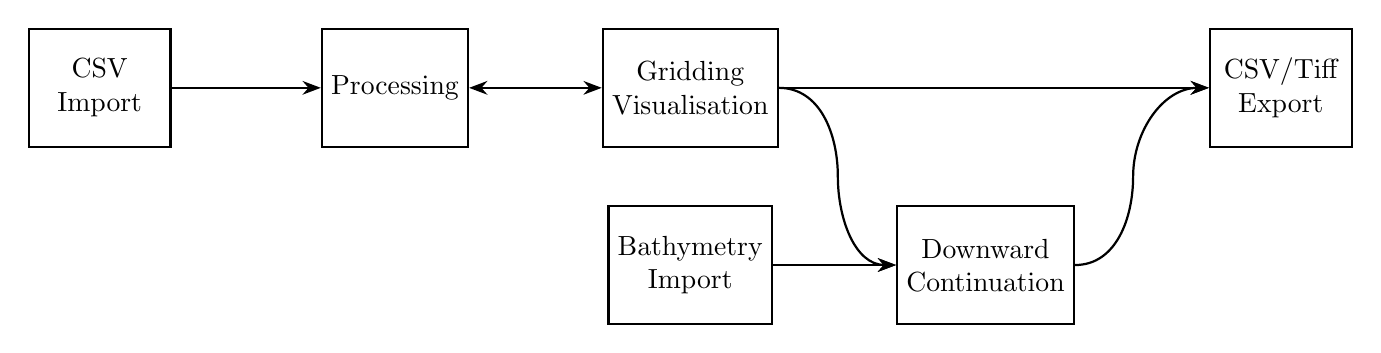
\begin{tikzpicture}[scale=1.5]
		\begin{scope}[every node/.style={rectangle,thick,draw,align=center, minimum width=1.8cm, minimum height=1.5cm}]
			\node (CI) at (0,0) {CSV\\Import};
			\node (P) at (2.5,0) {Processing};
			\node (GI) at (5.,0) {Gridding\\
				Visualisation};
			\node (BI) at (5.,-1.5) {Bathymetry\\
				Import};
			\node (TE) at (10,0) {CSV/Tiff\\Export};
			\node (DC) at (7.5,-1.5) {Downward\\Continuation};
		\end{scope}
		
		\tikzstyle{arrow} = [thick,<->,>=Stealth,color=black]
		\draw [arrow] (P) -- node[anchor=north] {} (GI);
		
		\tikzstyle{arrow} = [thick,->,>=Stealth,color=black]
		\draw [arrow] (CI) -- node[anchor=north,align=center] {} (P);
		\draw [arrow] (GI) -- node[anchor=north] {} (TE);
		\draw [arrow] (BI.east) -- node[anchor=south] {} (DC.west);
		
		\draw [arrow] (GI.east) to[out=0, in=90] (6.25, -0.75) 
		to[out=270, in=180] (DC.west);
		
		\draw [arrow] (DC.east) to[out=0, in=270] (8.75, -0.75) 
		to[out=90, in=180] (TE.west);
		
	\end{tikzpicture}
	\caption{
		The software implements a processing pipeline that reads INFOMAR's magnetometry data, processes, visualizes it and eventually exports the result.
		An additional branch provides an opportunity to import bathymetry data to interpolate the downward filed at the provided altitudes.
	}
	\label{fig:pipline}
\end{figure*}



\section{The processing pipeline}
The processing pipeline (see Fig.~\ref{fig:pipline}) consists of four key steps which is importing data, processing, gridding and eventually exporting the result.
An experimental branch of downward continuing the estimated grid will be discussed in section~\ref{sec:downwardContinuation}.

\subsection{Data import}
Data can be imported through a file dialogue that could be opened within the drop-down menu {\em File}.
The software is targeted at INFOMAR's magnetometry data acquired through Marine Magnetics SeaLink and Bob software.
Therefore, we provide two custom imports that directly can process a majority of raw files created by either software.
For details on assumptions of the raw files we refer to section \ref{sec:SeaLinkImport} and \ref{sec:BobImport}.
The imported surveys appear in a tree structure on the left-hand site of the main window (see \ref{fig:tree_import}).

\begin{remark}
	We note that the import of large \verb|*.txt| or many \verb|*.XYZ| files might take some time. Upon completion the imported surveys will appear in the file tree.
\end{remark}



\begin{figure}
	\centering
	\includegraphics[width=.9\textwidth]{./pic/DropDownMenuImport.png}
	\caption{
		Raw files can be imported through a file dialogue that will be triggered by the drop-down menu {\em File}.
	}
	\label{fig:drowdown_import}
\end{figure}

\begin{walkthrough}
	The surveys \verb|CV16_02_23042016.txt| and \verb|CV16_04_06082016.txt| have already been recorder using Marine Magnetics Bob software while \verb|CV_16_01| was still recorded using SeaLink.
	Accordingly, both \verb|CV16_02_23042016.txt| and \verb|CV16_04_06082016.txt| are present as single file, while \verb|CV_16_01| is a folder containing a nested \verb|raw| folder with the individual lines.
\end{walkthrough}

\begin{figure}
	\centering
	\includegraphics[width=.9\textwidth]{./pic/TreeMainWindow.png}
	\caption{
		The imported surveys appear in a tree structure on the left-hand site of the main window.
		The files contained in a SeaLink folder will appear under the node of its corresponding survey \texttt{CV\_YY\_NN}.
		Similar for surveys acquired with the Bob software will also appear as a single file within the corresponding node \texttt{CV\_YY\_NN}.
	}
	\label{fig:tree_import}
\end{figure}

\subsubsection{Marine Magnetics SeaLink import}
\label{sec:SeaLinkImport}

Surveys acquired using the Sealink acquisition software will be present as a folder named \verb|CV_YY_NN|, where YY denotes the year of the survey and NN the number of the survey.
The folder \verb|CV_YY_NN| itself should contain a folder called \verb|raw|.
Inside the \verb|raw|-folder are several files sharing the same filename but differ in their ending such as \verb|*.txt|, \verb|*.mag|, \verb|*.XYZ|.
The software is looking for files ending with \verb|*.XYZ|.

To deal with the huge heterogeneity among SeaLink files the software assume a minimal standard of the imported files which will be outlined in the following.
This has to be ensured by the user or the custom csv-import (see \ref{sec:customCSVimport}) might be tried.

Currently, the software has two assumptions on the \verb|*.XYZ| files.
First, a homogeneous number of columns within each file is expected since at the moment the software is not able to process files whose number of columns changes mid-file.

Second, the software assume the existence of the following columns names:\newline
\verb|/Date,Time,Field_Mag1,Longitude,Latitude|.
First, we note that due to Sealinks exported file structure the name has to be without \verb|/Date| without a space.
Moreover, \verb|/ | with a space is used to filter for mid-file headers, i.e. all lines starting with \verb|/ |  will be ignored.
Second, we note that the Software will probe for \verb|UTM_Easting,UTM_Northing|.
If these columns are not present in the raw file they will be estimated form \verb|Longitude,Latitude|.
An example how a \verb|*.XYZ| files is suppose to be formatted is given in listing \ref{lst:SeaLinkSnippet}.

If both requirement are meet, the user can open a file dialogue through the dropdown menu \verb|File| (see Fig.~\ref{fig:drowdown_import}).
Within the spawned file dialogue the user can select either directly the desired survey folder \verb|CV_YY_NN| or its contained \verb|raw| folder and all files matching the requirements above will be imported.
\begin{listing}[htbp]
\lstinputlisting[
	basicstyle=\ttfamily\scriptsize,
	captionpos=b,
	caption={Preview of a raw SeaLink CSV file.},
	label={lst:SeaLinkSnippet},
	]{./data/snippetSealink.txt}
\end{listing}

\subsubsection{Marine Magnetics Bob import}
\label{sec:BobImport}
Surveys acquired using the Bob acquisition software will be present as a single file named \verb|CV_YY_NN_*.txt|, where YY denotes the year of the survey and NN the number of the survey and \verb|*| denotes an arbitrary number unique for the survey.

Currently, the software has two assumptions on the \verb|CV_YY_NN_*.txt| files.
First, a homogeneous number of columns within each file is expected since at the moment the software is not able to process files whose number of columns changes mid-file.

Second, the software assume the existence of the following columns names:\newline
\verb|Reading_Date,Reading_Time,Magnetic_Field,Longitude,Latitude,UTM_Easting,UTM_Northing|.
An example how a \verb|*.XYZ| files is suppose to be formatted is given in listing \ref{lst:BobSnippet}.




\begin{listing}[htbp]
	\lstinputlisting[
	basicstyle=\ttfamily\scriptsize,
	captionpos=b,
	breaklines=true,
	caption={Preview of a raw Bob CSV file.},
	label={lst:BobSnippet},
	]{./data/snippetBob.txt}
\end{listing}


\subsubsection{Custom CSV import}
\label{sec:customCSVimport}
The software also support processing custom, meaning files different formatted than Marine Magnetics Bob or SeaLink \verb|*.csv| files.
However, there are a couple assumptions on the \verb|*.csv| which has to be ensured by the user.
\begin{itemize}
	\item The file has to contain in every row the same amount of columns.
	\item Special characters encoding a missing value or any other surprising event have to be replace with an empty string, i.e. an empty field.
	\item The file has to contain a header naming the columns.
\end{itemize}
A dialog, which can be spawn upon clicking on \enquote{From custom csv} in the drop-down menu (see Fig.~\ref{fig:tree_import}), will ask for the file that is to be imported and which columns to use for what purpose.
\begin{figure}
	\centering
	\includegraphics[width=.5\textwidth]{./pic/Custom_CSV_Import_Dialog.png}
	\caption{
		The dialog provides an interface to the user where he can denote which names column corresponds to entity, e.g. time, longitude, etc.
	}
	\label{fig:custom_scv_import_dialog}
\end{figure}


\subsection{Time series processing}
Next, we recommend inspecting the time-series through the \enquote{timeseries}-window, which can be opened through the dropdown menu {\em view}.
The \enquote{timeseries}-window facilitates two key tasks: displaying the time-series and manipulating it.
The time series itself can be displayed by clicking on \inlinegraphics{./../../ui_elements/icons/area-chart-icon.png}.
This also replicates the time-series on the main window and vice versa if \inlinegraphics{./../../ui_elements/icons/area-chart-icon.png} is clicked on the main window.
Moreover, this operation internally smooths the time series and calculates the residuals as the difference between the ambient field, estimated as a slow running mean, and the current field, estimated as a fast running mean.
The used window size of both means is preset upon preliminary work.
However, it can be adjusted through the text fields on the right-hand sight of either the main window ot the times series window. 
\begin{remark}
We note that this approach assumes a constant ambient field for the duration of the window~\cite{JOSS_paper}.
A diurnal correction using data from the Valencia observatory\footnote{\url{https://data.magie.ie/}} might be included in the future.
\end{remark}
Inside the plot, the time series could be investigated using zooming and panning.
The unprocessed time-series data might show huge negative spikes as depicted in Fig.~\ref{fig:scissorInterval}.
This is due to the fact that some raw data values are approaching $0\text{[nT]}$, probably during recovering the magnetometer.
The scissor tool \inlinegraphics{./../../ui_elements/icons/cut-scissor-icon.png} is designed to remove these intervals form the time-series.
The tool can be activated by clicking on the corresponding icon.
This allows the user to select a red rectangle by moving its edges, defining the interval that is to be excluded (see Fig.\ref{fig:processedTimeSeries}).
The rectangle can be adjusted until the selection is confirmed by clicking the scissor icon again and a final dialogue will confirm the decision.
We note that at the moment the visualisation will not refresh itself automatically.
This can be achieved by clicking again on \inlinegraphics{./../../ui_elements/icons/area-chart-icon.png}.
\begin{figure}
	\centering
	\includegraphics[width=.9\textwidth]{./pic/IntervalRemovalTimesieres.png}
	\caption{
		The imported raw times series might contain values approaching $0\text{[nT]}$, perturbing the calculated residuals.
		The \inlinegraphics{./../../ui_elements/icons/cut-scissor-icon.png} allows to remove an interval of undesired data points, configured as red rectangle.}
	\label{fig:scissorInterval}
\end{figure}

%\begin{walkthrough}
%	\verb|CV16_02| covers the 
%\end{walkthrough}

\begin{figure}
	\centering
	\includegraphics[width=.9\textwidth]{./pic/TimeSeriesWindow.png}
	\caption{
		A cleaned time-series using the \inlinegraphics{./../../ui_elements/icons/cut-scissor-icon.png} tool as depicted in Fig.~\ref{fig:scissorInterval}.
	}
	\label{fig:processedTimeSeries}
\end{figure}

\subsection{Anomaly grid processing}
The next step is the creation of the anomaly map.
This can be achieved upon selecting \inlinegraphics{./../../ui_elements/icons/drawingIcon.png}.
The initial result will look similar to Fig.~\ref{fig:initalAnomaly}.
\begin{remark}
	We note that the gridding step might take some time in particular if a high resolution is required.
\end{remark}
Generally, the visualization can be interacted with using panning and zooming.
Additionally on the right-hand side of the main window, various layers such as the backround map or the track lines can be enabled or disabled via the checkboxes and the scale of the anomaly can be adjusted between to be either linear and logarithmic.

This is due to the fact that at the moment the software interpolates the anomaly grid within the convex hull of the given data points.
\begin{figure}
	\centering
	\includegraphics[width=.9\textwidth]{./pic/InitalAnomalyMap.png}
	\caption{
		Gridding the processed time-series of \texttt{CV\_16\_01}, \texttt{CV\_16\_02} and \texttt{CV\_16\_04} will interpolate an anomaly map within the convex hull of the remaining data points.
		Outliers might cause artifacts as depicted.
	}
	\label{fig:initalAnomaly}
\end{figure}
Outliers, such as the single point located near the coast will cause undesired artifacts as shown in Fig.~\ref{fig:initalAnomaly}.
Those can be removed using the the scissor tool \inlinegraphics{./../../ui_elements/icons/cut-scissor-icon.png}.
Upon, activation the user can lasso-select an arbitrary set of points which will be removed.
The lasso is controlled by the user drawing a free-hand curve through left-clicking desired points on the map and subsequent closed upon deselecting \inlinegraphics{./../../ui_elements/icons/cut-scissor-icon.png} again.
Similar to cleaning time series, the selection can be confirmed or discarded in a final dialogue. 
This process is illustrated in Fig.~\ref{fig:lassoSelectAnomaly}.
\begin{figure}
	\centering
	\includegraphics[width=.9\textwidth]{./pic/LassoSelect.png}
	\caption{
		A free-hand curves (red dashed line) allows selecting undesired data points to be removed.
	}
	\label{fig:lassoSelectAnomaly}
\end{figure}
For a more fine selection, a polynomial select tool \inlinegraphics{./../../ui_elements/icons/object-select-icon.png} is provided.



\begin{figure}
	\centering
	\includegraphics[width=.9\textwidth]{./pic/ClippingTool.png}
	\caption{
		\inlinegraphics{./../../ui_elements/icons/object-select-icon.png} allows to clip a desired region using a polygon. The clipped region will be used for further processing and export.
	}
	\label{fig:polySelect}
\end{figure}

\begin{figure}
	\centering
	\includegraphics[width=.9\textwidth]{./pic/ClippedRegion.png}
	\caption{
		A zoomed view on the clipped region using the \inlinegraphics{./../../ui_elements/icons/object-select-icon.png} as indicated in Fig.~\ref{fig:polySelect}.
	}
	\label{fig:clipedRegion}
\end{figure}


\subsection{Export}

Finally, the processed anomaly grid can be exported over the drop-down menu {\em file} and then selecting either a text-based \verb|*.csv| or a \verb|*.tiff| based export.
The latter one exports a geotiff which could imported into any GIS software and further processes.

\section{Experimental: Downward continuation}
\label{sec:downwardContinuation}

\subsection{Bathymetry import}
\begin{remark}
	This section will be added once it is implemented in its finalized form.
\end{remark}


	
\printbibliography
\end{document}